\section{Cluster-based Map Abstraction}
\label{aha:mapabstraction}
The annotated graph we created in Section \ref{aha:computingclearance} is sufficient for computing a low-level strategy but this is inefficient for large problem size; we would prefer instead to express a more general strategy for navigating from the start to the goal position -- in terms of macro-operations.

We will achieve this by using a similar technique to that described in \cite{botea04} and divide our map into equally-sized adjacent sections called \emph{clusters}. This is a simple off-line process the results of which we outline in figure \ref{aha-fig:abstractgraph}a. If required, we can easily associate the location of an agent in the world with a cluster given a fixed cluster-size and the \emph{x,y} coordinates of the tile currently being occuppied.\\ \newline
Having thus decomposed the map we must now define transitions between each pair of adjacent clusters. HPA* proceeds by identifying \emph{entrances} between clusters, which are defined as contiguous areas between two adjacent lines of tiles, $l1$ and $l2$, that represent the border between clusters $c1$ and $c2$. For $e$ to be valid, it must respect a few key conditions:
\begin{enumerate}
\item{An entrance cannot span an area larger than the size of the border between two adjacent clusters.}
\item{The tiles in each cluster along the common border must be contiguous (no breaks) and symmetrical (ie. for each tile in $l1$ there exists an equivalent tile in $l2$.)}
\item{An entrance must contain no (hard) obstacle tiles.}
\end{enumerate}
Each entrance is associated with a particular \emph{size} (the length of the maximally sized contiguous area) and \emph{orientation} (either veritcal or horizontal depending on the nature of the adjacency) and represented in the abstract graph by one or two transition points, depending on the size of the entrance. \\ \newline
We apply a similar idea but take a single transition point: the pair of nodes which maximise the clearance value for a given capability. We compute this latter metric by taking the minimum clearance among each node pair in the entrance area and selecting the largest value from the resultant set. Each transition is represented in the abstract graph by a pair of nodes and an undirected edge of weight 1.\\
We proceed in this way for each available capability and annotate each resultant abstract edge with the clearance and capability values used to find it. We do not need to add any annotations to our abstract nodes; it is sufficient to define the length and traversal requirements of the corridor connecting them.  Figure \ref{aha-fig:abstractgraph} highlights this process. On the left we present two adjacent clusters, while on the right are the three entrances identified and their respective transition points. \emph{E1} and {E2} are discovered using single-terrain capabilities, while \emph{E3}, which spans the whole border area, is discovered using a more complex multi-terrain capability. Note that \emph{E3} shares the same the location on the low-level map with \emph{E1}; this is common where the latter capability used to identify entrances is a superset (ie. includes all terrains) of the former; in these cases, we re-use any existing abstract nodes. If the existing abstract nodes are already connected we also attempt to re-use the edge between them by checking if the existing edge is traversable using the capability and maximal clearance values of the new. In our example \emph{E3} represents a wider corridor than \emph{E1} so we add a new edge to the abstract multi-graph. \\ \newline

Our final step to complete the abstraction involves connecting each abstract node to every other in the local cluster. We achieve this by using AA* to search for the optimal path between each pair of nodes for all available capabilities and agent sizes. Once a path is found we insert a new undirected edge into the abstract graph to connect the two nodes using the path distance as its cost and annotating it with the capability and clearance parameters used by AA* to find the solution. To avoid edge duplication when pathfinding inside each  cluster we will order from lagest to smallest the set of available agent sizes which we pass as clearance parameters to AA*. We also order the capability parameters we pass to AA* from simplest (those containing the least number of terrains) to most complex (the capability corresponding to the set of all terrains). The intuition here is that if a traversable optimal-length path exists between two nodes we would like to re-use it instead of adding more edges to the graph. We thus present our complete map decomposition approach in  algorithm \ref{aha-alg:buildabstraction}.

\input algorithms/alg_buildabstraction

\subsection{Optimising Abstract Graph Size}
A possible risk with our decomposition algorithm is that as the number of terrains in the environment increase the size of the abstract graph will become larger and larger and in turn, result in degraded planning performance. One strategy for addressing this problem is to use the concept of dominance relationships to minimise the number of edges we add to the abstract graph. The idea is simple: if two nodes are connected by multiple edges with overlapping capabilities, we prefer to keep the edge with the largest clearance and simplest traversal requirements, irrespective of comparative differences in length. A reasonable analogy we could draw at this point is to compare the way off-road vehicles opportunistically use roads where possible even if an off-road route (or trail) might exist which has a smaller distance cost. We prefer roads because are smoother to drive on and have other benefits such less wear and tear, better fuel consumption per kilometer ratio and so on. Of course, opting for a lower-quality abstraction in this way does have an effect on the quality of the computed solutions, but as we will show in our experimental analysis, the differences are reasonably small and the solutions still near-optimal for our test data. The best choice here depends on the requirements of the specific application to which the algorithm is applied; it is a classic tradeoff between performance vs space.

Figure \ref{aha-fig:abstractgraph} shows the results of our abstraction technique on the toy map presented earlier. In \ref{aha-fig:abstractgraph}c we show the final abstraction result; we were able to represent a 2-terrain map with 100 nodes and 350 edges using just 13 nodes and  23 edges. In \ref{aha-fig:abstractgraph}d we show a low-quality abstraction. In this trival example we could only reduce the abstract edge count by 2 (in cluster \emph{C1}) but this is an atypical result as we will later demonstrate.

\begin{figure}[htbp]
        \caption{\emph{Entrance Building Examples} }
        \begin{center}
                        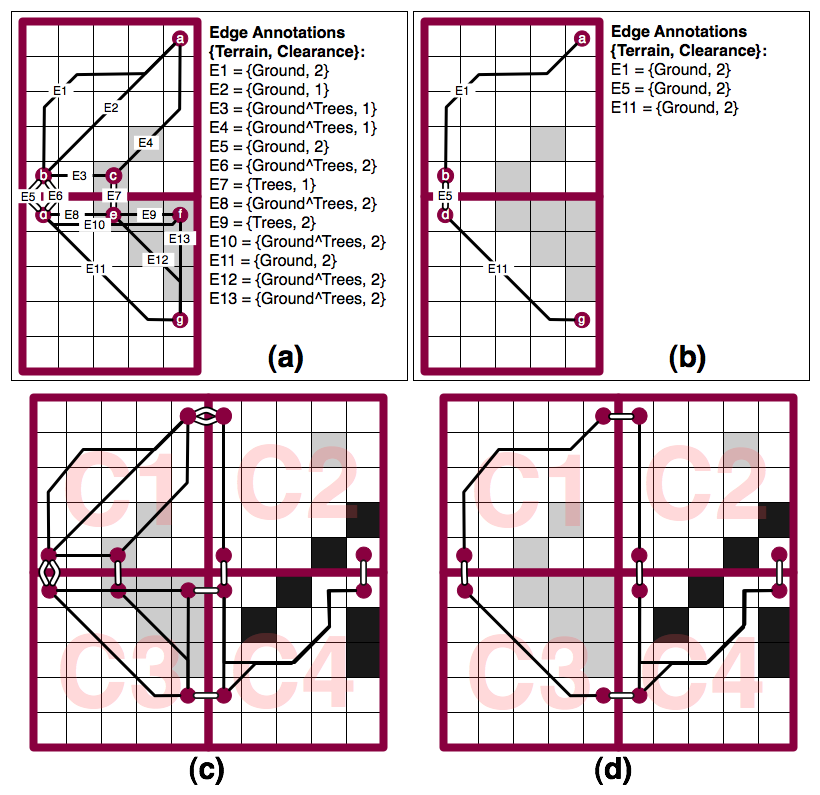
\includegraphics[scale=0.25]{diagrams/clusters_and_entrances.png}
        \end{center}
        \label{aha-fig:abstractgraph}
\end{figure}

The size of the resultant abstract graph is hard to characterise because it depends on the features of the environment we are analysing. Complex maps with may terrains and smaller cluster sizes will result in larger graphs. Less terrains or larger cluster sizes will produce fewer nodes and edges. In any case, we will require an additional 2 annotations for each abstract edge. The total number of annotations in the abstract graph is therefore linear in the number of edges. Meanwhile, the total number of annotations can be re-stated as: 

\begin{equation}
N*2^t/2 - |N_{HO}| + 2*|E_{abstract}|
\label{aha-eq:totalannotations}
\end{equation}

Where $|E_{abstract}|$ is the size of the set of edges in the abstract graph.

